% !TEX root = ../Article.tex
%\chapter{Testing}
\chapter{Testing and use case implementation}
\label{ch:testing}
%In this chapter we will perform tests on the smart card regarding cryptographic performance and proof of concept implementation to evaluate the proposed solutions from the previous chapter. The tests will help us determine if smart cards are a valuable addition to mobile security or if they lack the power to function properly in a mobile device environment.
In this chapter we describe the tests we designed and ran to evaluate the cryptographic capabilities and performance of the smart cards, communication and compatibility between smart cards and Android, and possible technical problems that may present themselves when using smart cards. The implementation and tests took a lot of resources and time as it was difficult to debug problems that occurred on the smart cards and in the third party libraries we used. The remaining time was spent on implementing and testing the binding protocol we described in section \ref{sec:bindingcardandphone}.

% !TEX root = ../Article.tex
\section{Setup}
In order to do research on how smart cards can have an impact on mobile data security and to perform an evaluation on how effective they are we need to have a proper test environment. We define ``proper test environment'' as an environment as close to reality as possible.
\subsection{Equipment}
\label{sec:equipment}

\paragraph{Test device}\mbox{}\\
The device we will be using for deploying the applications and performing tests on is considered to be a mid-range device. The device is a Sony Xperia M2 Aqua smartphone running Android 5.1.1 with the following relevant specifications:
\begin{itemize}
    \item Chipset: Qualcomm MSM8926-2 Snapdragon 400
    \item CPU: Quad-core 1.2 GHz Cortex-A7
    \item RAM: 1 GB
\end{itemize}
More information on the specifications of the phone can be found on  \newline
GSMArena.com \cite{sonym2}.

\paragraph{Java smart card}\mbox{}\\
We will be using two types of smart cards. The first type is a micro SD memory card (IDCore 8030 MicroSD card) as shown in figure \ref{fig:msdcard} produced by Gemalto. The reasoning for using this card for testing is that Gemalto delivers ready-to-use cards along with a framework for communicating with them. The cards we will be using have nothing pre-installed on them and we can freely deploy custom applications to the card. In order to use the provided framework we need a key provided by Gemalto which has a validity period of 120 days.

The second type of card we will be using is a plain hybrid smart card (ref. figure \ref{fig:nfccard}) with no pre-installed software which is also provided by Gemalto along with a standard card reader. In this case we are not reliant on the framework provided by Gemalto as Android has built in support for NFC communication in the standard SDK.

Both types of card are able to run the same application and thus makes it very convenient when comparing their performance against each other.

\iffalse %COMMENT

\subsection{Java card application}\mbox{}\\
The cards we have supports java card 2.2.2 and this is the version we will target. A natural question is "Why don't we target java card 3 and above?". Smart cards used for banking or handling other highly confidential data needs to be evaluated under the Common Criteria \cite{commoncriteria} standards. Potentionally we may handle confidential data and as a result we want smart cards with a Evaluation Assurance Level (EAL) 4 or above. Achieving EAL4 or above is an expensive and long process and the relatively few products have this certification. The micro SD card we have access to are certified with EAL5+, but only supports java card 2.2.2 \cite{gemaltoidgo8030}.

%TODO EAL list

A natural question we need to ask ourselves is: "Do we want Java card 3?"



\paragraph{Development environment}\mbox{}\\
In order to develop applications for the smart cards we will be using Eclipse 3.2 with java development kit version 1.6.45. In order to develop smart card applications more easily we will use the Eclipse-JCDE plugin \cite{eclipseJCDE} which provides a virtual runtime environment along with build tools.

We will be using GlobalPlatformPro (GP) \cite{globalplatform} to deploy and manage applets on the physical smart cards. GP is a command line tool and is compatible with our hybrid Gemalto card with reader as well as the micro SD card.

To test the smart card application that is deployed on the physical cards (without going through an Android application) we will be using pyApduTool \ref{pyapdutool}. pyApduTool is a tool for sending APDUs to a smart card through a card reader or memory card reader and lets us observe how the card behave when receiving and transmitting data.

\paragraph{Goal}\mbox{}\\
The goal of the smart card application was to create an autonomous and easy to extend platform for future tests. This resulted in an application split into three parts.

\paragraph{Initialization}\mbox{}\\
As described in section \ref{sec:javacard} all javacard applications must implement the method \texttt{Install}. \texttt{Install} invokes the constructor of the smart card and this is where all variables that need initialization are initialized. For instance if the smart card application needs to generate keys or random numbers this is where it is done as the constructor will be invoked only once. All buffers that needs to be used should also be initialized here to avoid allocating memory everytime the application is used.

\paragraph{Data processing}\mbox{}\\
In the mandatory \texttt{Process} method (refer to section \ref{sec:javacard}) all data processing takes place. First a built in method in the javacard API, \texttt{selectingApplet()}, is invoked. This method checks if the incoming APDU is a SELECT APDU and acts accordingly. If the incoming APDU is not a SELECT APDU the incoming APDU is copied to a new buffer for easier data manipulation. Next we use a switch statement switching over the second byte, INS, to determine which instruction we want to perform. After processing the data and performing the work we want to do (sign data, encrypt, etc.) we copy our response to the outgoing buffer.

\paragraph{Finalization}\mbox{}\\
At the end of the \texttt{Process} invokation we invoke the \texttt{Send} method which takes the data in the outgoing buffer, package it for sending and send it as a response APDU.

\paragraph{The result}\mbox{}\\
What we end up with is a test plattform where we are only concerned with declaring variables, initializing variables and writing code for the specific test case. Listing \ref{lst:pseudoCard} shows pseudocode for the java card application with the extendable areas highlighted.


\begin{lstlisting}[caption=Pseudo code for javacard test application., label=lst:pseudoCard,escapechar=!]
public class cardApplication extends Applet implements ExtendedLength{

    !\colorbox{highlight}{//Variable declarations}!

    private cardApplication() {
    	!\colorbox{highlight}{//Variable initialization}!
    }

    public void process(APDU apdu) {
    	//Process incoming APDU
        if (selectingApplet()) {
			return;
		}
        buff = apdu.getBuffer();

    	switch(buff[ISO7816.OFFSET_INS]){
            case 0x00:
            case 0x01:
            !\colorbox{highlight}{...}!
            case 0xff:
            default:

    	}
    	Send(apdu);
    }

    private void send(APDU apdu) {
    	//Package outgoing buffer
    	//Send response APDU
    }
}
\end{lstlisting}

\fi %UNCOMMENT

\iffalse %COMMENT

\subsection{Android application}
\paragraph{IDE}\mbox{}\\
Android Studio \cite{androidIDE} is the official IDE for Android application development. Android Studio is based on IntelliJ IDEA \cite{intelliJIDEA} and provides many automated tools for building, packaging and publishing Android applications.
\paragraph{3rd party libraries}\mbox{}\\
As mentioned in section \ref{sec:equipment} Gemalto provides a java library, IDGo800, for using their smart cards.

\begin{aquote}{Gemalto.com \cite{GemaltoIDGo800}}
"IDGo 800 for Mobiles is a cryptographic middleware that supports the Gemalto IDPrime cards and Secure Elements on Mobile platforms: Contact and contactless smart cards, MicroSD cards, UICC-SIM cards, embedded Secure Elements (eSE) and Trusted Execution Environment (TEE)."
\end{aquote}

The part of IDGo800 SDK we are interested in is very small and enables us to send custom APDUs to micro SD smart cards.

We will be using the "android.nfc" package in order to communicate with NFC smart cards. This package is included in the standard Android SDK which in turns means that all Android devices with a NFC reader and minimum API level 9 \cite{androidNFCminSDK} can use our library.

\paragraph{Application}\mbox{}\\
We used the same approach on the Android application as on the smart card application; an autonomous and easy to extend plattform for tests. This resulted in a new library, "smartcardlibrary",  which sole purpose is to transmit APDUs as easily as possible.

Smartcardlibrary has two main functions:
\begin{enumerate}
    \item{Communicate with NFC card}
    \item{Communicate with mSD card}
\end{enumerate}

To send APDUs to a smart card,\texttt{NFCSmartcardController} or\\ \texttt{MSDSmartcardController} (depending on smart card type) must be instantiated and the application must know the application identifier of the smart card application. Further the current activity must implement\\ \texttt{NfCSmartcardControllerInterface} or \texttt{MSDSmartcardControllerInterface} (depending on smart card type) in order to be notified when the transaction is complete. Listing \ref{lst:NFCLibraryExample} shows an example implementation on how an activity may utilize the library for NFC smart cards.

\begin{lstlisting}[caption=Java code example showing how to send and receive commands to a NFC smart card., label=lst:NFCLibraryExample,escapechar=å]

public class PayloadActivity extends AppCompatActivity implements NFCSmartcardControllerInterface {
    NFCSmartcardController nfcscc;
    ...

    private void initNFCCommunication(){
        if(nfcscc == null) {
            nfcscc = new NFCSmartcardController(this, this);
        }

        String AID = "0102030405060708090007";
        String hexMessage = "95404F3FB1";
        String cmd = "06";
        String p1 = "00";
        String p2 = "00";

        nfcscc.sendPayloadDataToNFCCard(AID, cmd, p1, p2, hexMessage);
    }

    å@Overrideå
    public void nfcCallback(final String completionStatus){
        if(!completionStatus.equals("OK")){
            return;
        }
        StorageHandler stHandler = new StorageHandler(getApplicationContext());
        String response = stHandler.readFromFileAppDir(FilePaths.tempStorageFileName);
    }
}

\end{lstlisting}

In order for the library to perform an asyncronous transaction the library will temporary save the responses from the cards to a file only accessible by the running application. To retrive the data the current activity should use the included \texttt{StorageHandler} class as used in listing \ref{lst:NFCLibraryExample}. The library also provides the class, \texttt{Converter}, for converting between Strings, hex and byte arrays.

Figure \ref{fig:package} shows how the library is structured and the entry point for applications is through the packages:

\begin{itemize}
    \item com.master.henrik.controller
    \item com.master.henrik.statics
    \item com.master.henrik.shared
\end{itemize}



\begin{figure}[h!]
  \caption{Library package diagram.}
  \label{fig:package}
  \centering
    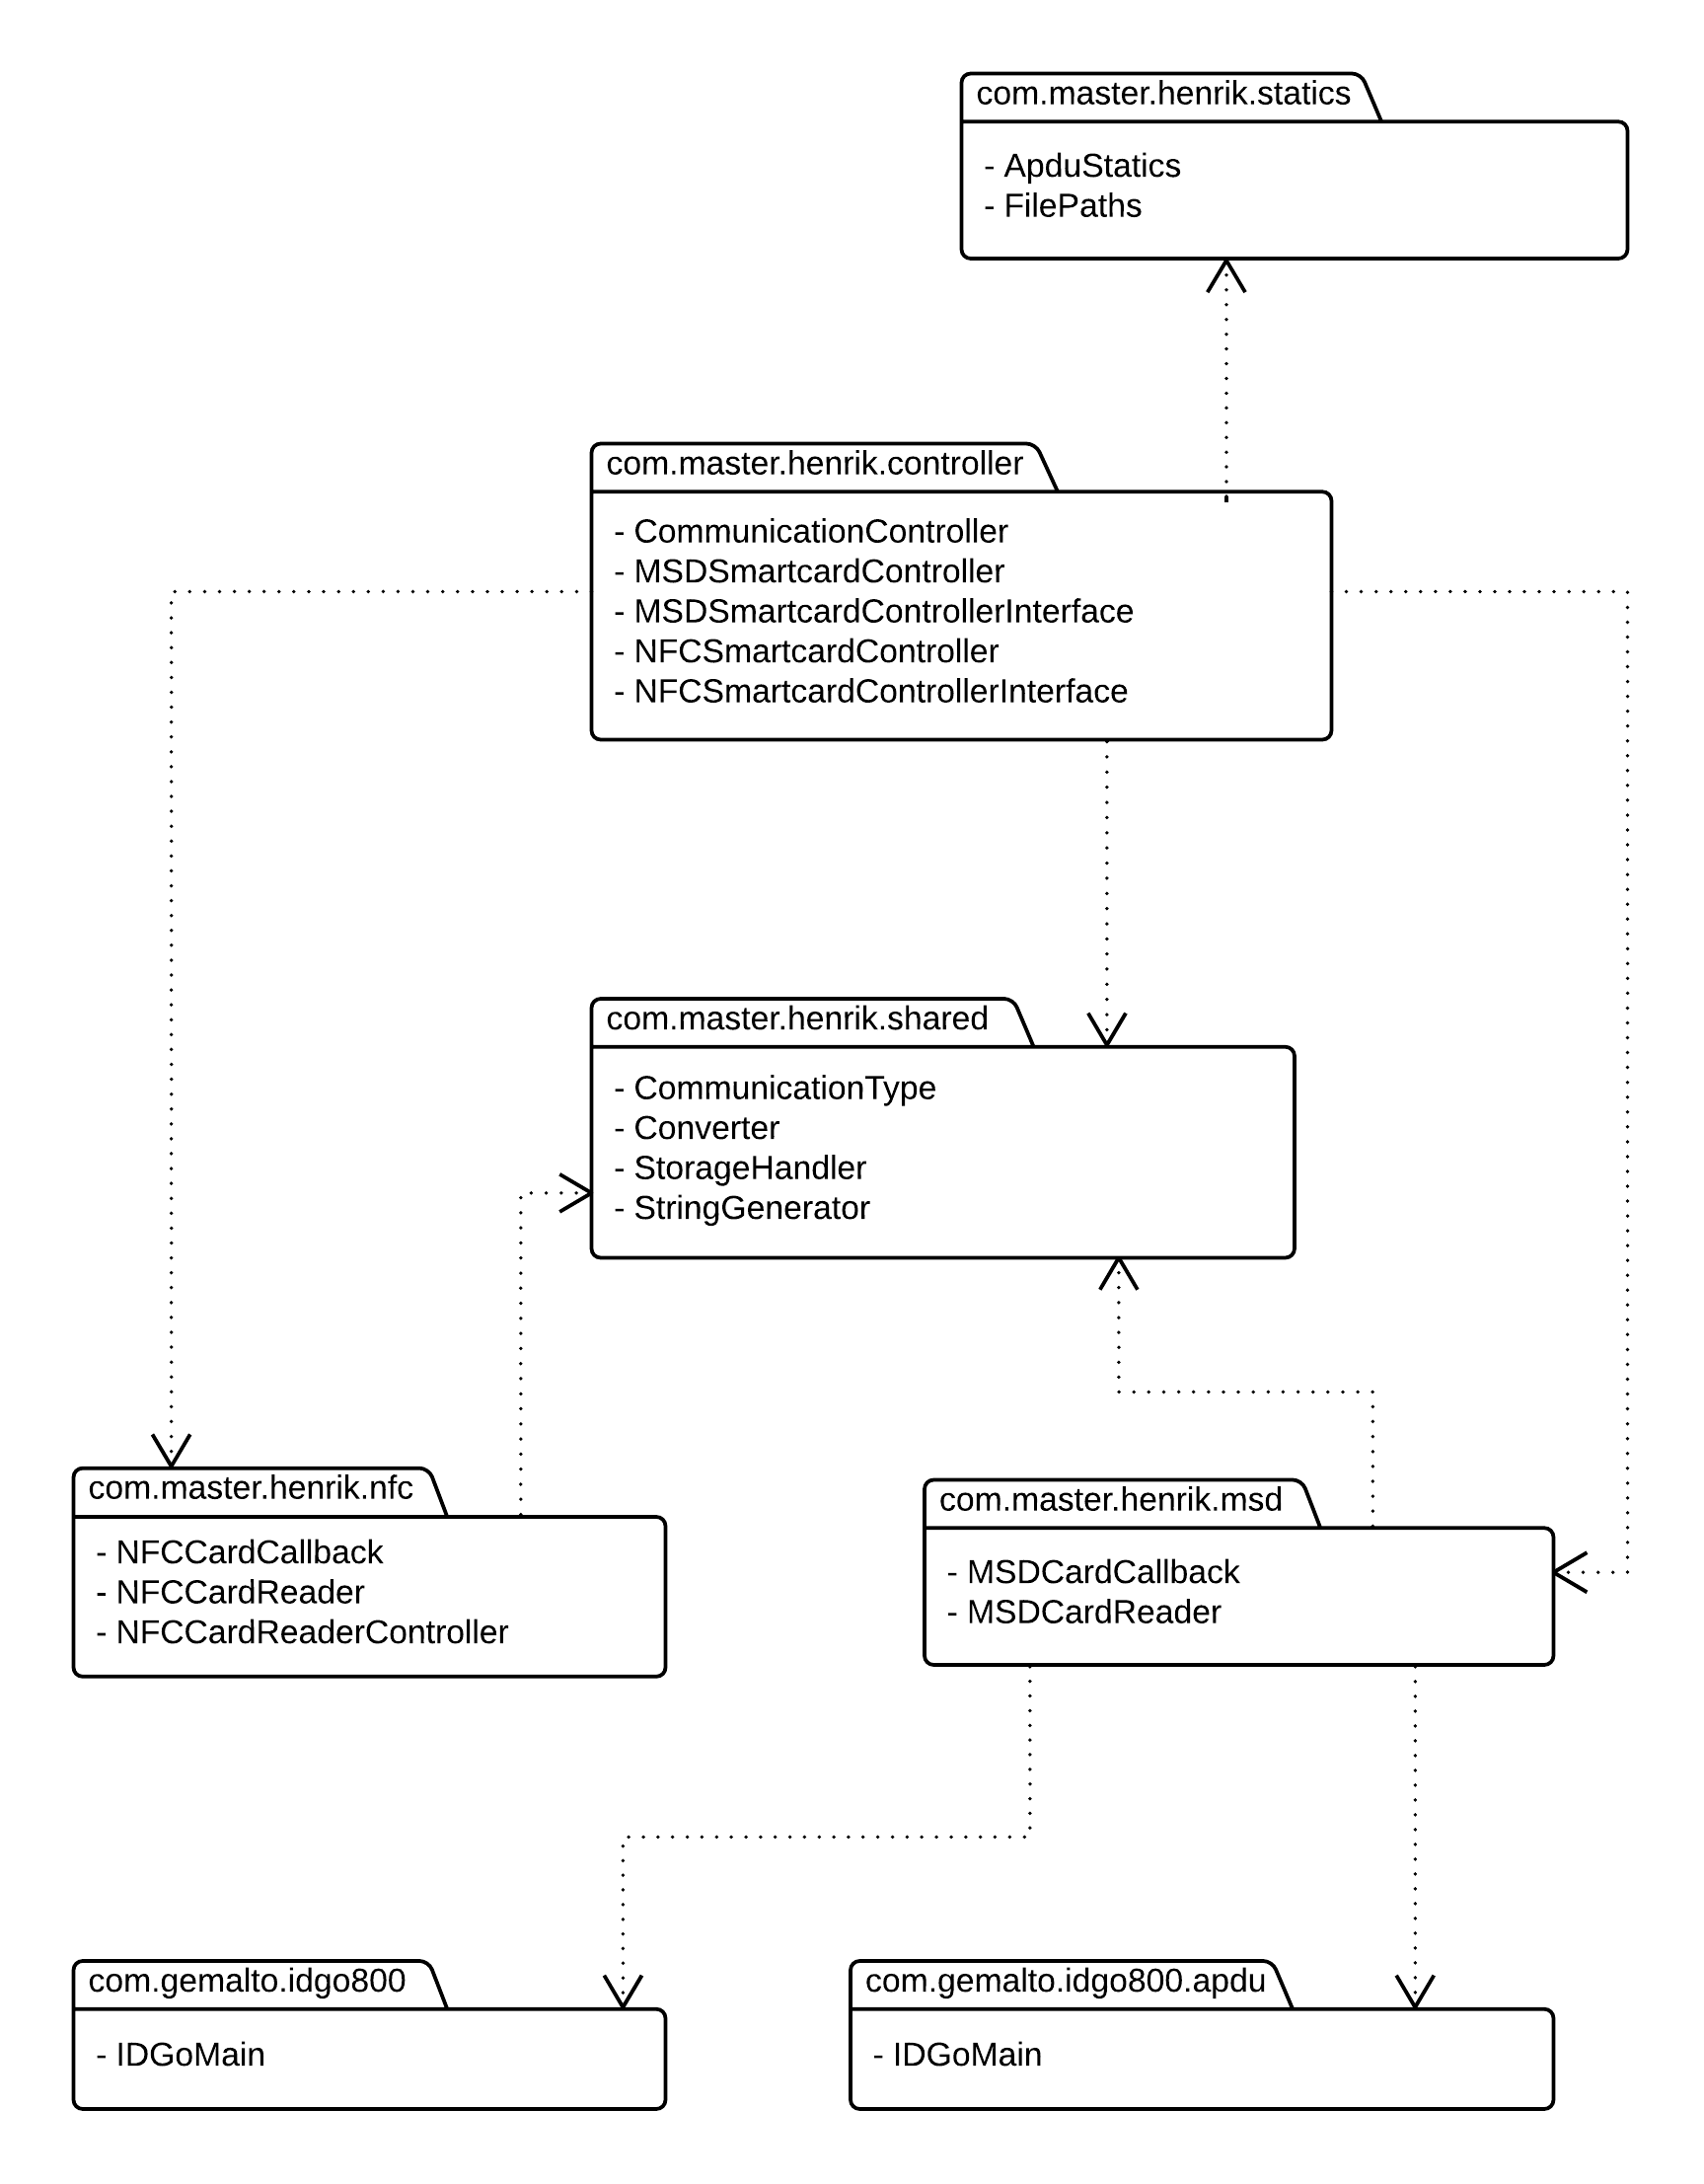
\includegraphics[width=0.95\textwidth]{images/package2.png}
\end{figure}

\fi %UNCOMMENT

\subsection{Limitations}
\label{sec:limitationsMSD}
When we started testing the implementation it became evident that the micro SD smart card we had did not support extended APDU. As a result we are not able to perform tests that involve micro SD cards and extended APDU.


% !TEX root = ../../Article.tex
\section{Data Transfer Speed}
\subsection{Description and Motivation}
Transfer speed is a very vital for part of the smart card interaction. If the smart card application or the transportation layer is incapable of handling large amounts of the data we will need to take that into account when examining the usability of smart cards. In order to test and eliminate as many variables as possible the smart card is programmed to receive data, copy the incoming data to the buffer and send the exact same data in return. Figure \ref{fig:nfcDataflowTest} describes this process using an NFC card as a platform for the Java Card Applet.

\begin{figure}[h!]
  \caption{Data flow of data transfer speed test for NFC.}
  \label{fig:nfcDataflowTest}
  \centering
    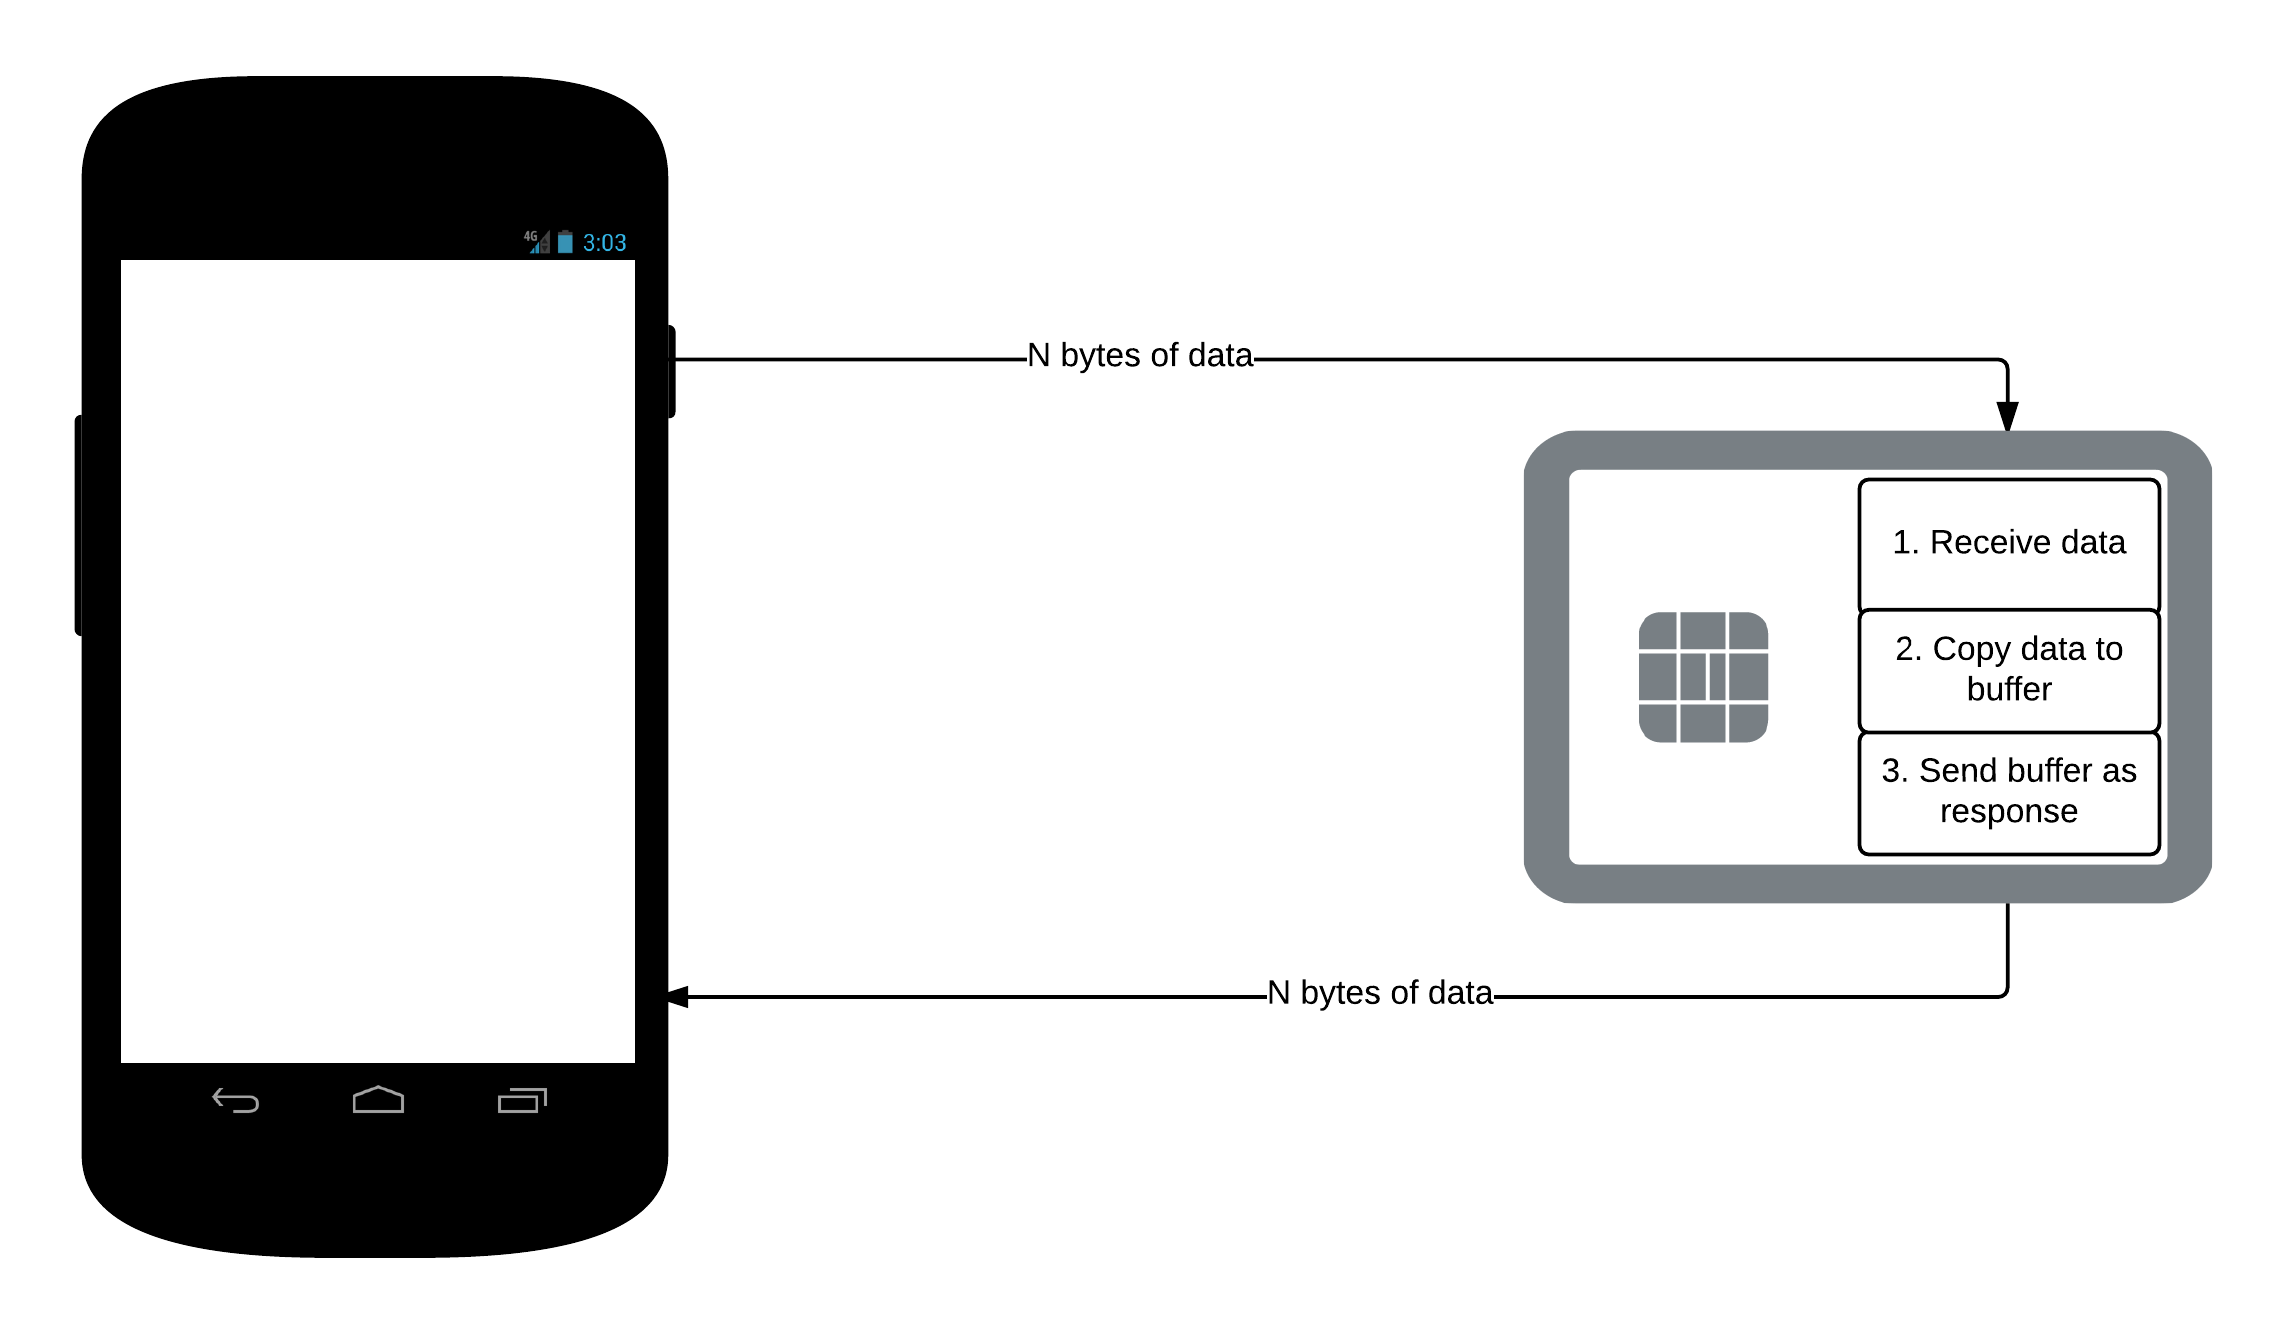
\includegraphics[width=0.95\textwidth]{images/NFCTransferTest.png}
\end{figure}

\subsection{Tests and Results}
\paragraph{NFC}\mbox{}\\
\begin{table}[h!]
\caption{Table of NFC transfer speed test.}
\label{tbl:nfcspeed}
\centering

    \begin{tabular}{ | l | r | r | r |}
        \hline
        \thead{Data size (byte)}
        & \thead{T1}
        & \thead{T2}
        & \thead{T3} \\ \hline

        10000 & 3,8s & 4,1s & 3,6s \\ \hline
        100000 & 41,3s & 35,0s & 24,7s \\ \hline
        1000000 & 602,1s & 361,3s & 235,1s \\ \hline

    \end{tabular}

\end{table}

%\vspace{1cm}
\begin{figure}[h!]

    \caption{Graphical representation of table \ref{tbl:nfcspeed}.}
    \label{fig:nfcgraph}
    \begin{tikzpicture}
        \centering
            \begin{axis}[
                width  = 0.85*\textwidth,
                height = 8cm,
                major x tick style = transparent,
                ybar=2*\pgflinewidth,
                bar width=14pt,
                ymajorgrids = true,
                ylabel = {Running time (seconds)},
                xlabel = {Data size (byte)},
                symbolic x coords={10000, 100000, 1000000},
                xtick = data,
                scaled y ticks = false,
                enlarge x limits=0.25,
                ymin=0,
                legend cell align=left,
                legend style={
                        at={(1,1.05)},
                        anchor=south east,
                        column sep=1ex
                }
            ]
                \addplot[style={bblue,fill=bblue,mark=none}]
                    coordinates {(10000, 3.89) (100000, 41.29) (1000000, 602)};

                \addplot[style={rred,fill=rred,mark=none}]
                     coordinates {(10000, 4) (100000, 35) (1000000, 361)};

                \addplot[style={ggreen,fill=ggreen,mark=none}]
                     coordinates {(10000, 3.6) (100000, 24) (1000000, 235)};

                \legend{T1 Configuration,T2 Configuration,T3 Configuration}


            \end{axis}
    \end{tikzpicture}
\end{figure}


\newpage
\paragraph{Micro SD}\mbox{}\\
T1 configuration, from NFC was dropped when testing transfers speed for micro SD as it became clear from previous tests on NFC that T1 is vastly inferior to T2 and T3. A non-asyncronous (not using streams) Android application is not representative of the "real-world" and we decided on not pursuing further test results using this configuration.

T2 configuration consist of the Android application sending data to the smart card application using frames of size 255 byte until all data is sent. Simultaneously the responses are written to an internal file using FileOutputStream (provided by the standard Java library).

We were not able to test T3 configuration as explained in section \ref{sec:limitationsMSD}.

\begin{table}[h!]
\caption{Table of micro SD transfer speed test.}
\label{tbl:msdspeed}
\centering

    \begin{tabular}{ | l | r | r |}
        \hline
        \thead{Data size (byte)}
        & \thead{T2}
        & \thead{T3} \\ \hline

        10000  & 3,18s & N/A s \\ \hline
        100000 & 16,14s & N/A s \\ \hline
        1000000 & 142s & N/A s \\ \hline

    \end{tabular}

\end{table}


\newpage
\subsection{Conclusion}
From table \ref{tbl:nfcspeed} and figure \ref{fig:nfcgraph} we can learn that we are able to optimize the data transfer and processing speed between the Android application and the NFC card. It is also clear that when we are transmitting low amounts of data there is virtually no difference between the configurations; T1, T2 and T3. The differences are more prominent when the data amounts increase. Even though we achieved an improvement of approximately 60 \% from T1 to T3 when sending 1 MB of data, the process is still time consuming.

If we compare the test results for T2 configuration on the NFC card and micro SD card we can clearly see an improvement on the micro SD card. The micro SD card had a ~60 \%  better running time over the NFC card when sending 1 MB of data. Although we were not able to test configuration T3 on the micro SD card, results point in the direction of micro SD cards having better performance than NFC cards. We are not able to confirm this and thus cannot be treated as a fact.

Even though we are able to optimize and improve data transfer speeds, we are still very far from transferring and processing large amounts of data quickly. We have to take this into account when evaluating areas of use for the smart card. Transfer and processing speed rules out many areas concerning large amounts of data, such as full data encryption.


% !TEX root = ../../Article.tex
\section{Symmetric-key Cryptography}
\label{sec:symmetricTest}
\subsection{Description and Motivation}
We want to discover the encryption abilities on the smart card and decide if it is feasible to let the smart card handle the encryption of confidential data. From the smart card documentation we know that we are able to use AES to encrypt data, but we do not know how long it will take to encrypt the data. We will need to perform a run time tests with different amounts of data in order to determine the performance of the smart card.

\subsection{Test setup}
The framework we are using is designed around extended APDU and the test platform we have designed in Java Card utilizes extended APDU. As a result we are not able to use the micro SD cards (as described in section \ref{sec:limitationsMSD}) and we will be using the NFC smart cards.

The encryption algorithm we will use is AES cipher algorithm with block chaining (CBC). The version of Java Card that we are using along with our smart cards limits us to using 128 bits keys and no padding. More specifically the only working AES algorithm from javacard is \texttt{ALG\_AES\_BLOCK\_128\_CBC\_NOPAD}, even though the Java Card documentation for \texttt{Cipher} supports more algorithms \cite{javacardCipher}. Others have encountered the same discrepancy \cite{javacardCipherFail} suggesting that only three of the twelve supported algorithms works, but there exists no official information on the issue.

\texttt{ALG\_AES\_BLOCK\_128\_CBC\_NOPAD} is as the name suggest an algorithm with no padding. The block size the AES algorithm expects is 16 byte and as a result we will need to pad the data ourselves on the mobile device.

\subsection{Results}
% !TEX root = ../Article.tex

\begin{table}[h!]
\caption{Table of AES encryption speed test.}
\label{tbl:AESSpeed}
\centering

    \begin{tabular}{ | l | r |}
        \hline
        \thead{Data size (byte)}
        & \thead{Elapsed time} \\ \hline

        10000  & 20,18s \\ \hline
        32000  & 61,81s \\ \hline
        100000 & 183,78s \\ \hline
        1000000 & 1835,49s \\ \hline

    \end{tabular}

\end{table}

\begin{figure}[h!]

    \caption{Graphical representation of table \ref{tbl:AESSpeed}.}
    \label{fig:nfcgraph}
    \begin{tikzpicture}
        \centering
            \begin{axis}[
                width  = 0.85*\textwidth,
                height = 8cm,
                major x tick style = transparent,
                ybar=2*\pgflinewidth,
                bar width=14pt,
                ymajorgrids = true,
                ylabel = {Running time (seconds)},
                xlabel = {Data size (byte)},
                symbolic x coords={16, 10000, 32000, 100000, 1000000},
                xtick = data,
                scaled y ticks = false,
                enlarge x limits=0.25,
                ymin=0,
                legend cell align=left,
                legend style={
                        at={(1,1.05)},
                        anchor=south east,
                        column sep=1ex
                }
            ]
                \addplot[style={bblue,fill=bblue,mark=none}]
                    coordinates {(16, 0.15) (10000, 20.62) (32000, 61) (100000, 183) (1000000, 1835)};
            \end{axis}
    \end{tikzpicture}
\end{figure}

\subsection{Conclusion}
From the test results we can learn that encrypting data on the NFC smart card takes a lot of time. Encrypting 1MB of data uses approximately 30 minutes, which from a real world perspective is an unacceptable amount of time. Using the NFC smart card for full encryption of user data is in other words not achievable and we will need to look for other options for encryption.

Encrypting 16 bytes of data uses 0,15 seconds. A use for the encryption capabilities on the smart card may be to encrypt small amounts of data such as GPS coordinates. GPS coordinates can be represented by only 16 bytes (depending on accuracy). One could also imagine that we will only need to encrypt parts of a document, and as long as we keep the data size small we can let the smart card do the encryption.


% !TEX root = ../../Article.tex
\section{Binding card and mobile device}

